%%%%%%%%%%%%%%%%%%%%%%%%%%%%%%%%%%%%%%%%%
% baposter Portrait Poster
% LaTeX Template
% Version 1.0 (15/5/13)
%
% Created by:
% Brian Amberg (baposter@brian-amberg.de)
%
% This template has been downloaded from:
% http://www.LaTeXTemplates.com
%
% License:
% CC BY-NC-SA 3.0 (http://creativecommons.org/licenses/by-nc-sa/3.0/)
%
%%%%%%%%%%%%%%%%%%%%%%%%%%%%%%%%%%%%%%%%%

%----------------------------------------------------------------------------------------
%	PACKAGES AND OTHER DOCUMENT CONFIGURATIONS
%----------------------------------------------------------------------------------------

\documentclass[a0paper, portrait]{baposter}

\usepackage[font=small, labelfont=bf]{caption} % Required for specifying captions to tables and figures
\usepackage{booktabs} % Horizontal rules in tables
\usepackage{relsize} % Used for making text smaller in some places
\usepackage{enumitem} % Use for small margin bullet lists
\graphicspath{{figures/}} % Directory in which figures are stored

\definecolor{bordercol}{RGB}{40,40,40} % Border color of content boxes
\definecolor{headercol1}{RGB}{186,215,230} % Background color for the header in the content boxes (left side)
\definecolor{headercol2}{RGB}{80,80,80} % Background color for the header in the content boxes (right side)
\definecolor{headerfontcol}{RGB}{0,0,0} % Text color for the header text in the content boxes
\definecolor{boxcolor}{RGB}{186,215,230} % Background color for the content in the content boxes Use c1d0e1 to rem

\begin{document}

\background{ % Set the background to an image (background.pdf)
\begin{tikzpicture}[remember picture,overlay]
\draw (current page.north west)+(-2em,2em) node[anchor=north west]
{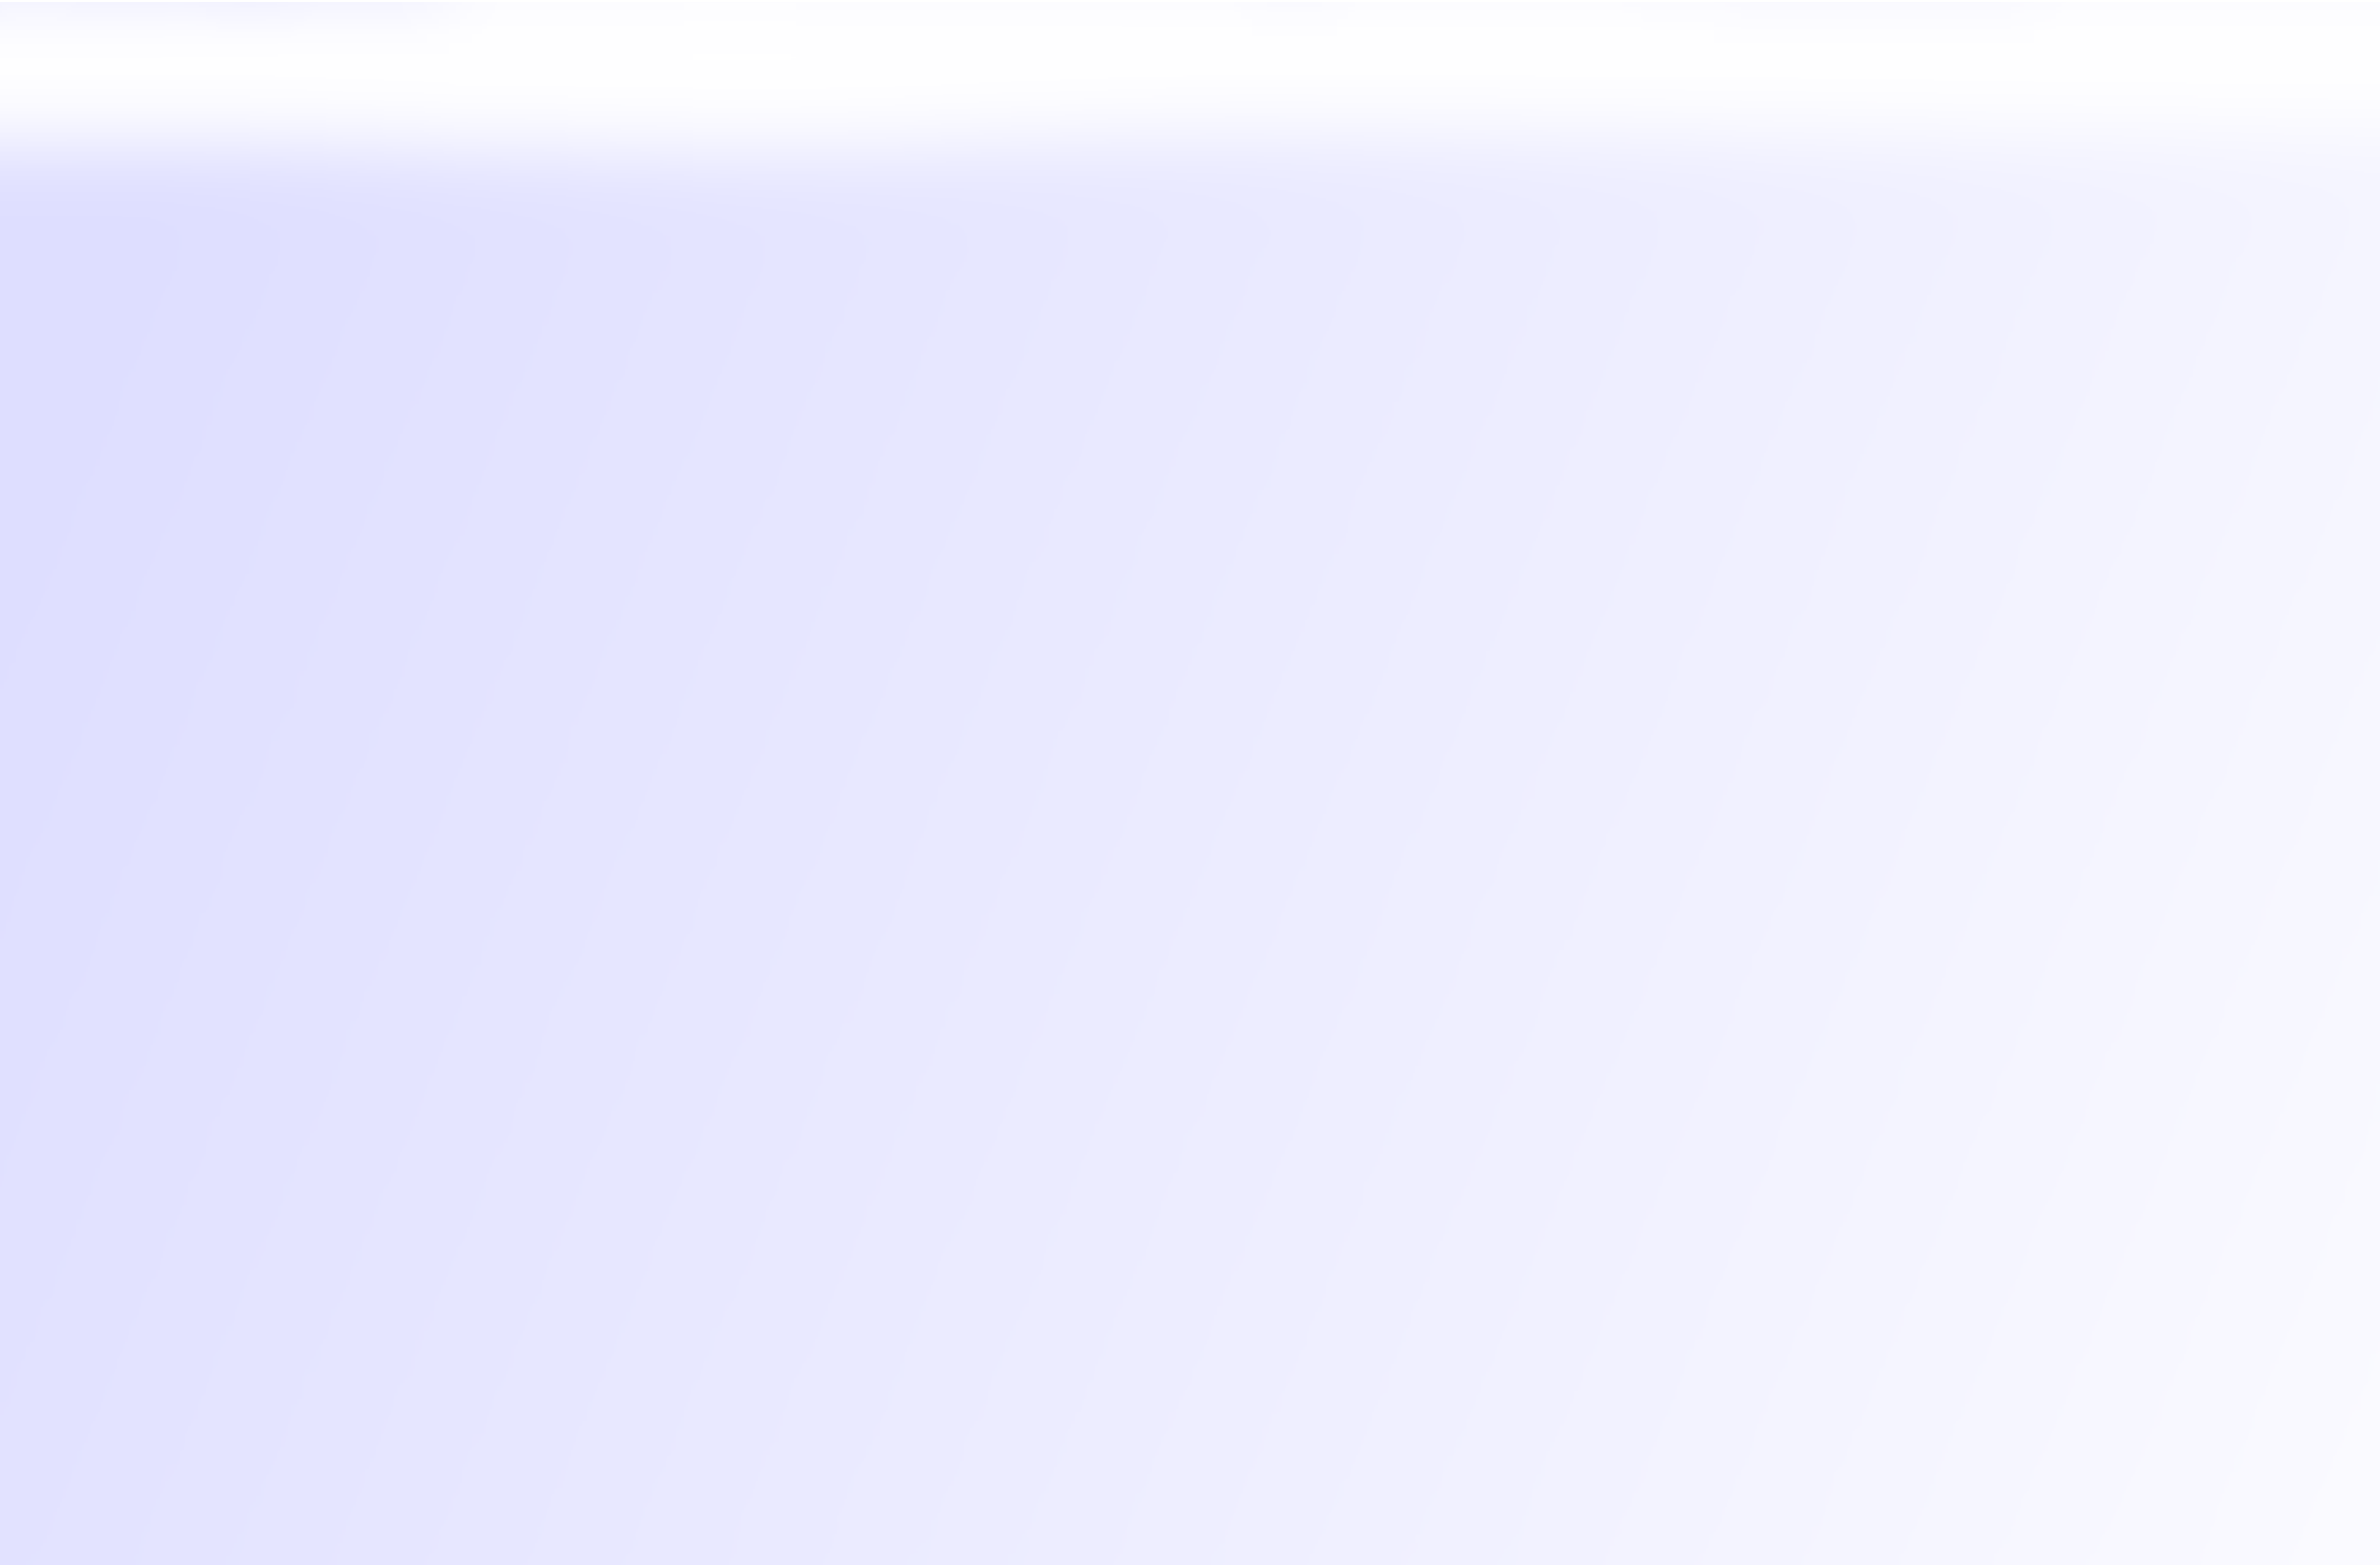
\includegraphics[height=1.1\textheight]{background}};
\end{tikzpicture}
}

\begin{poster}{
	grid=false,
	borderColor=bordercol, % Border color of content boxes
	headerColorOne=headercol1, % Background color for the header in the content boxes (left side)
	headerColorTwo=headercol2, % Background color for the header in the content boxes (right side)
	headerFontColor=headerfontcol, % Text color for the header text in the content boxes
	boxColorOne=boxcolor, % Background color for the content in the content boxes
	headershape=roundedright, % Specify the rounded corner in the content box headers
	headerfont=\Large\sf\bf, % Font modifiers for the text in the content box headers
	textborder=rectangle,
	background=user,
	headerborder=open, % Change to closed for a line under the content box headers
	boxshade=plain
} 
%
%----------------------------------------------------------------------------------------
%	TITLE AND AUTHOR NAME
%----------------------------------------------------------------------------------------
%
{
\includegraphics[scale=0.6]{uob-logo.eps}} % left logo
{\sf\bf\huge Untangling the chromatin conformation \\ of the \textit{GNG12-AS1/DIRAS3} locus} % Poster title
{\vspace{0.5em} Stephen Richer, Giuseppina Pisignano, Adele Murrell, Dorothy Buck \\ 
{\vspace{0.5em} s.richer@bath.ac.uk}} 
{
\includegraphics[scale=0.11]{qrcode}} % right logo

%----------------------------------------------------------------------------------------
%	INTRODUCTION
%----------------------------------------------------------------------------------------

\headerbox{Introduction}{name=introduction,column=0, row=0}{

\begin{itemize}[leftmargin=*]
\item Here we investigate chromatin organisation at the \textit{GNG12-AS1/DIRAS3} locus.
\item \textit{DIRAS3} is maternally imprinted and these genes are reciprocally expressed throughout the cell cycle. 
\item SiRNA knock-down of exon 1, but not exon 7, leads to \textit{up-regulation} of \textit{DIRAS3} \cite{Stojic2016}.
\item What role does chromatin organisation play in this negative gene non-autonomy? 
\end{itemize}

\begin{center}
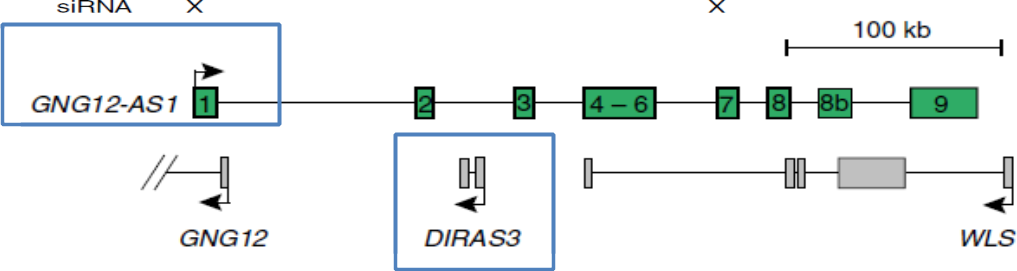
\includegraphics[width=1.0\linewidth]{gng12-locus}
\captionof{figure}{The \textit{GNG12-AS1} genomic locus.}
%(chr1: 68,297,971 - 68,668,670)
\end{center} 
}

%----------------------------------------------------------------------------------------
%	MATERIALS AND METHODS
%----------------------------------------------------------------------------------------

\headerbox{Materials and Methods}{name=methods,column=0,below=introduction}{

\begin{description}
\item[Capture HiC] Generate high-resolution chromatin conformation maps of the \textit{GNG12-AS1} locus in HB2 (mammary epithelial) and MCF7 (breast cancer) cell lines.
\item[Bioinformatics] Compare TAD structure and assess changes in contact frequency between cancer and non-cancer cell lines.
\end{description}

\begin{center}
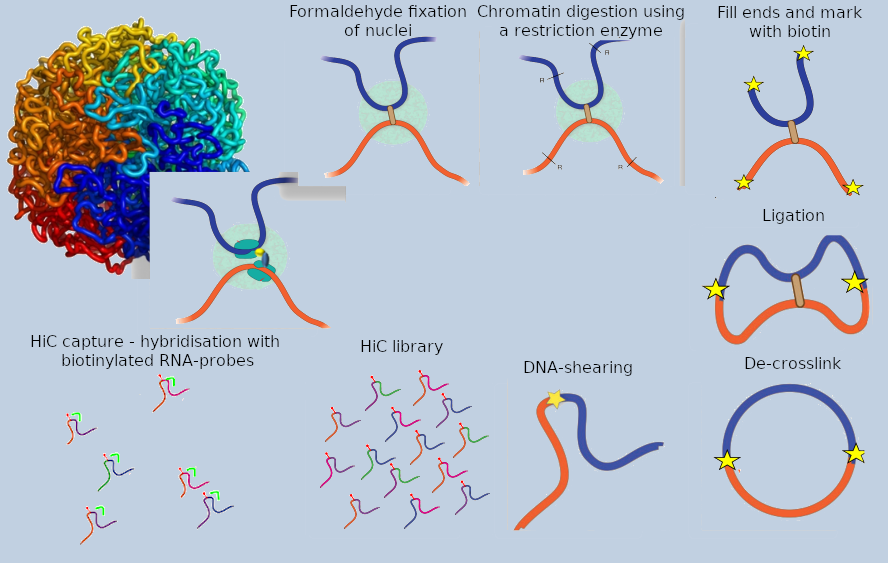
\includegraphics[width=1.0\linewidth]{hic_technique}
\captionof{figure}{Overview of capture HiC protocol.}
\end{center}

}

%----------------------------------------------------------------------------------------
%	CONCLUSION
%----------------------------------------------------------------------------------------

\headerbox{Future work}{name=conclusion,column=0,below=methods}{

\begin{itemize}[leftmargin=*]
\item Create 3D visualisation of DNA looping based on HiC interaction map.
\item What are biological implications of reduction in interaction frequency, between HB2  and MCF7, at \textit{GNG12-AS1} locus?
\item Investigate unexpected changes up-down and down-stream of \textit{GNG12-AS1} locus.
\item Allele specific HiC to study effect of imprinting on chromatin organisation. 
\item Refine methods to robustly compare TAD changes between samples.
\end{itemize}

}

%----------------------------------------------------------------------------------------
%	REFERENCES
%----------------------------------------------------------------------------------------

\headerbox{References}{name=references,column=0,
	below = conclusion, above = bottom}{

\smaller % Reduce the font size in this block
\renewcommand{\section}[2]{\vskip 0.05em} % Get rid of the default "References" section title
\nocite{*} % Insert publications even if they are not cited in the poster

\bibliographystyle{unsrt}
\bibliography{poster-abr} 
}

%----------------------------------------------------------------------------------------
%	RESULTS 1
%----------------------------------------------------------------------------------------

% To reduce this block to 1 column width, remove 'span=2'
\headerbox{Chromatin organisation and TADs at \textit{GNG12-AS1}} {
	name = results1, span = 2, column = 1}{ 
\vspace{1em}
%------------------------------------------------
\begin{center}
\includegraphics[width=1.0\linewidth]{GNG12_AS1_DIRAS3_ontad_sum_3000_count}
\captionof{figure}{
HiC interaction map, summed across two replicates, for HB2 (top) and MCF7 (bottom) cell lines .
Matrices were binned at 3000bp, normalised for read depth and corrected using iterative correction.
TADs were called independently for each replicate using OnTAD \cite{An2019}.
Current methods show some inconsistency in TADs identified between replicates.
However, TAD boundaries align well with CTCF binding sites and reveal a complex hierarchical structure.
These TADs likely represent a consensus set of domains that exist among the cell population and across the cell cycle.
}
\end{center}
%------------------------------------------------
}

%----------------------------------------------------------------------------------------
%	RESULTS 2
%----------------------------------------------------------------------------------------
% To reduce this block to 1 column width, remove 'span=2'
\headerbox{Chromatin conformation changes between HB2 and MCF7} {
	name = results2, span=2, column = 1, 
	below = results1, above = bottom}{
\vspace{1em}
%------------------------------------------------

\begin{center}
\includegraphics[width=1.0\linewidth]{GNG12_AS1_DIRAS3_HB2_WT_vs_MCF7-logFC}
\captionof{figure}{
Log\textsubscript{2} fold-change of MCF7 over HB2 interaction frequencies, binned at 5000bp.
Red represents an increase in interaction frequency in MCF7 and blue represents a decrease.
Differential interactions were called using diffHiC \cite{Lun2015}.
Significant changes were defined as those with absolute log\textsubscript{2} fold-change $>$ 2 and FDR $<$ 0.01.
Broad regions of reduced contact frequency, in MCF7, were detected approximately 1.5 megabases downstream of \textit{GNG12-AS1} (purple), near \textit{PDE4B} (red), \textit{MIRE1} (black) and \textit{SGI1P} (yellow).
Increases in contact frequency, in MCF7, were also detected between \textit{LRRC7} (green) and a number of regions approximately 500 kilobases upstream of \textit{GNG12-AS1}.
}
\end{center}

}

\end{poster}

\end{document}